% Author: David Sanchez-Jacome

\chapter{Introduction and objectives} \label{chap:intro}

\section{Integrated circuits} \label{sec:integrated_circuits}

Electronic integrated circuits (ICs) have revolutionized the last decades due to their ability to integrate a vast number of functionalities into a small physical space, leading to significant reductions in cost, power consumption, and increases in speed and reliability.
With the invention of the transistor this solid-state device replaced bulky and less efficient vacuum tubes, enabling miniaturization \cite{bardeen_transistor_1948}.
This in turn led to the development of the first integrated circuit \cite{kilby_invention_1976, riordan_crystal_1997}.
This innovation allowed for the fabrication of multiple interconnected electronic components on a single semiconductor substrate, paving the way for complex systems on a chip.
At the same time, continuous advancements in lithography enabled the fabrication of increasingly smaller and more densely packed transistors, as described by Moore's Law, leading to exponential growth in computing power and functionality \cite{moore_cramming_2006}.
The development of CMOS (complementary metal-oxide-semiconductor) technology offered low power consumption and high integration density, making it the dominant technology for modern ICs \cite{wanlass_low_1967}.
CMOS made possible the invention of the microprocessor \cite{noauthor_announcing_nodate}.
This milestone integrated the central processing unit (CPU) of a computer onto a single chip, enabling the personal computer revolution and the proliferation of digital technologies.
Building on the density offered by CMOS, the focus has also expanded from monolithic integration on a single chip to system-level integration through advanced packaging \cite{tummala_fundamentals_2001}.
This approach allows multiple, often specialized, integrated circuits (known as 'chiplets') to be combined into a single compact and high-performance package, pushing the boundaries of miniaturization and functionality even further \cite{naffziger_22_2020}.
These advancements have collectively driven the ubiquity of ICs across diverse fields by enabling complex information processing, communication, and control in increasingly smaller, cheaper, and more energy-efficient devices.

In parallel to the growth of electronic hardware, software has played a pivotal and increasingly significant role in the trajectory of integrated circuits from their inception to their pervasive presence in modern life.
Initially, software was crucial for the design, simulation, and testing of these nascent integrated circuits.
As IC complexity grew exponentially, sophisticated Computer-Aided Design (CAD) tools, which are fundamentally software applications, became indispensable for engineers to manage the intricate layouts and functionalities of microchips \cite{lienig_fundamentals_2021}.
Beyond the design phase, software is the very essence that provides ICs with purpose and enables their application in everyday activities.
This is possible due to layered architecture adopted for software buildup \cite{tanenbaum_structured_2013} (see Figure~\ref{fig:ch1-abstraction_layers} for an example of software layers).
At the lowest level, firmware and microcode reside directly within the IC itself, controlling the fundamental hardware operations and basic functionalities \cite{hennessy_computer_2017}.
The operating system acts as an intermediary layer, managing the IC's resources and providing a standardized platform for software applications \cite{tanenbaum_modern_2009}.
Device drivers enable the operating system to communicate with specific hardware components, translating generic commands into device-specific instructions \cite{corbet_linux_2005}.
Libraries and Application Programming Interfaces (APIs) offer collections of reusable code and standardized interaction methods, abstracting hardware complexities for application developers \cite{gamma_design_1994}.
Finally, applications are the user-facing software programs that perform specific tasks, leveraging the underlying software stack and the capabilities of the ICs to deliver their intended functionalities.

\begin{figure}
	\begin{center}
		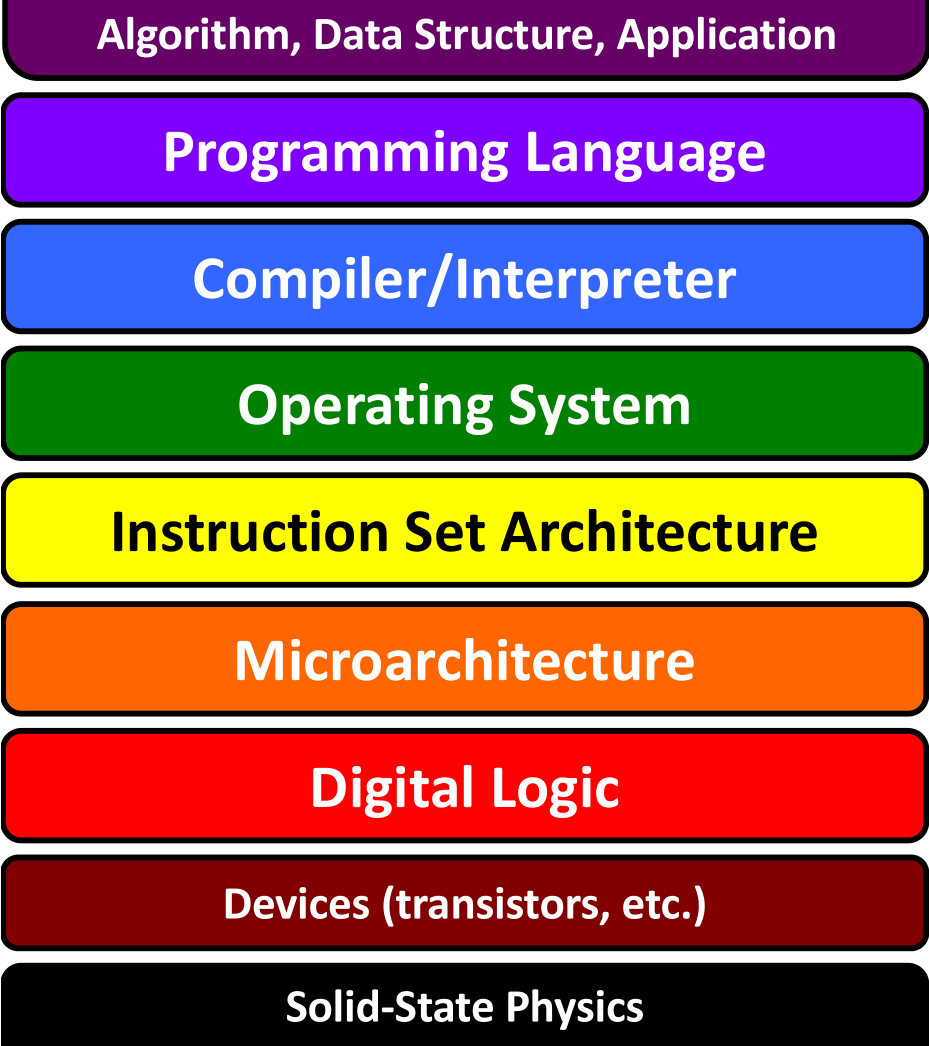
\includegraphics[width=0.35\textwidth]{figures/ch1-abstraction_layers.png}
	\end{center}
	\caption{Diagram of software abstraction layers of a typical computer system \cite{ondich_cs_2022}}\label{fig:ch1-abstraction_layers}
\end{figure}

Consequently, software stacks have democratized ICs because of their ability to translate physical semiconductor variables into human-readable instructions that can be reused and built upon.
In other words, while integrated circuits provide the physical substrate for computation and control, it is the multifaceted layers of software that orchestrate their operation, manage their resources, and ultimately translate their capabilities into the diverse array of technologies that underpin our daily lives.
The advancements in software have been unavoidably linked to the increasing power and versatility of ICs, creating a symbiotic relationship between them that continues to drive technological progress.

\section{The case for programmable integrated photonics} \label{sec:photonics_motivation}

While electronic ICs have undeniably transformed society, photonic integrated circuits (PICs) have gained significant interest and research focus due to their potential to overcome fundamental limitations of electronics and enable entirely new functionalities \cite{soref_past_2006,ye_review_2013,baets_silicon_2017}.
The motivation stems from several key factors.
Photonics inherently offers significantly higher bandwidth and lower latency for data transmission compared to electronics.
Indeed, the vast global infrastructure built upon optical fiber has demonstrated the immense capacity and efficiency of transmitting information using light.
This success naturally creates a compelling need to develop integrated photonic technologies that can efficiently interface with optical fiber and manipulate these optical signals using PICs.
As light propagates at higher speeds and with less loss in optical fibers and waveguides, PICs have become ideal for applications requiring massive data throughput, such as AI/ML data center and high-performance computing interconnects \cite{khani_sip-ml_2021,li_silicon_2015,zhou_development_2018}.
In terms of power consumption, optical communications and analog signal processing can be more energy-efficient than their electronic counterparts in certain applications, particularly over long distances (more than a few meters).
Photons do not carry an electrical charge, thus eliminating resistive losses and reducing power consumption in interconnects.
Light signals also provide immunity to electromagnetic interference (EMI) which gives photonic circuit a significant advantage in, otherwise noisy, electrical environments.
It's important to note that PICs can also be reconfigured through software just like electronic ICs, which enables them to tackle several real-life problems.
The latter fact makes them attractive for applications in microwave photonics \cite{chen_silicon_2017,marpaung_integrated_2019}, Lidar/Radar \cite{hashemi_review_2022,serafino_toward_2019}, or aerospace \cite{hsu_free-space_2022}, where signal integrity is paramount.
PICs also offer high sensitivity and precision for applications in environmental monitoring (e.g., gas and chemical sensing) \cite{chrostowski_silicon_2012}, biomedical diagnostics (e.g., lab-on-a-chip devices) \cite{fathpour_silicon_2011}, and precision metrology (e.g., optical gyroscopes) \cite{weimann_silicon_2017,khial_nanophotonic_2018}.
Likewise, reconfigurable PICs have also emerged as a promising platform for realizing complex and scalable quantum computing and communication networks \cite{harris_large-scale_2016,sibson_integrated_2017}.
All in all, similarly to electronic ICs, PICs allow for the integration of numerous optical components onto a single chip, leading to smaller, more robust, and potentially lower-cost devices.
This miniaturization facilitates the deployment of photonic technologies in a wide range of applications that demand increasingly better speed, bandwidth, power efficiency, and sensitivity specs.

In a context were most of PICs are tailored for a single application, multipurpose programmable PICs based on recirculating meshes represent a significant advancement in integrated photonics.
They have garnered considerable research interest over the last decade due to their unique capabilities and potential to revolutionize various applications.
These circuits distinguish themselves through their ability to be reconfigured for diverse functionalities on a single chip, offering a level of versatility that is highly desirable in modern photonic systems \cite{bogaerts_programmable_2020,capmany_programmable_2020,perez_multipurpose_2017}.
The key distinct feature of these PICs is their architecture, which typically consists of an interconnected network of fundamental programmable elements, such as Mach-Zehnder Interferometers (MZIs) or phase shifters, arranged in a grid-like mesh.
The crucial aspect is the "recirculating" nature of these meshes, allowing light to traverse the network through a wide set of configurations.
By precisely controlling each individual element, light can be routed along various paths and cycles within the mesh to be split, combined, and phase-shifted with remarkable flexibility.
This intricate control over the optical path allows for the implementation of a wide range of linear optical transformations, which form the foundation of many photonic applications.
Furthermore, the mesh structure is scalable within the application's insertion loss budget and reticle size limits.
Therefore, increasing the number of interconnected elements allows for the creation of more complex circuits capable of tackling increasingly complex tasks.

As stated previously, for integrated solutions to become ubiquitous they must be controllable via software and PICs are not the exception.
The importance of reconfigurable multipurpose PICs largely mirrors the motivations behind reconfigurable electronic platforms like field programmable gate arrays (FPGAs) and their synergy with software control.
Reconfigurability in PICs is crucial for application testing and prototyping because it enables a single PIC to be adapted to different functionalities or changing operational requirements after fabrication.
This is particularly valuable in dynamic environments such as telecommunications networks, where traffic patterns and service demands can fluctuate.
A reconfigurable PIC can be dynamically adjusted on-the-fly to service different scenario needs.
In the case of multipurpose PICs, hardware reconfigurability significantly speeds up the prototyping and development process of new photonic systems.
Instead of designing and fabricating a new chip for each iteration or different application, researchers and engineers can program this reconfigurable PIC to test various designs and functionalities.
This reduces time-to-market and lowers development costs.
Similarly, a reconfigurable PIC can be utilized for a wider range of applications or tasks compared to a fixed-function PIC.
This leads to better resource utilization and reduces the need for multiple specialized chips, potentially lowering overall system cost and complexity.
Following the footsteps of electronic ICs, where reconfigurability enables a higher level of abstraction and control through software, comes the impending need of developing software-defined photonics.
Just as software engineers can program electronic systems without needing deep knowledge of the underlying hardware, software interfaces for reconfigurable PICs allow users to define and control complex photonic functionalities through programming interfaces.
As a consequence, the motivation behind reconfigurable PICs, under this thesis framework, is to introduce a level of flexibility and programmability into the photonic domain that mirrors the power and versatility that software brings to electronic hardware.
This allows for greater adaptability, faster innovation, and broader applicability of photonic integrated circuit technology.
In other words, if multipurpose programmable PICs are empowered with a robust and user-friendly software stack, this programmability key holds the promise to unlock a vast array of possibilities on a single photonic hardware platform.

\section{Objectives} \label{sec:objectives}

Given that reconfigurable PICs are poised to become key enablers of several technologies due to the previously stated advantages, this thesis is developed under the framework of creating a commercially available multipurpose software-defined platform with a reconfigurable PIC at its core.
The aim is to create a technology stack that resembles those in the electronics world to drive and configure a reconfigurable photonic integrated circuit in order to expose a high-level application programming interface (API) to the final users of the platform.
From bottom to top, this stack should include the photonic core, the control electronics and the software that orchestrates everything and allows to map abstract high-level functionalities to the set of physical parameters driving the PIC.
With this, we aim to demonstrate how the development of a technology stack is the key to open the door for several applications powered by a single PIC architecture.

Specifically, the global objective of this industrial PhD is to contribute in creating the technology stack needed to operate a multipurpose programmable PIC and deliver it to a final user in the form of a commercial photonic processor.
The project started with the design, tape-out and submission to manufacturing of reconfigurable PICs based on hexagonal recirculating meshes.
It continued with the creation, development, and testing of a closed-loop control system that allows the configuration of the high-density programmable PIC while the manufacturing process was carried on by the foundry.
Once the semiconductor chips and the control-loop systems arrived from fabrication, the correct functioning of each one of these individual subcomponents was tested/debugged.
Subsequently, the entire photonic processor system had to be assembled ensuring correct communication and synchronization between its composing subsystems.
With the system ready, the activities focused on the development and testing of programming strategies and algorithms that allow the optimal configuration of the newly-developed high-density photonic processor.
Precisely, this part focused on developing a software layer to configure manually and automatically circuits with different functionalities on the photonic processor.
The final steps of the thesis dealt with the experimental demonstration of several applications using the same photonic processing platform: optical interconnects, reconfigurable beamsplitters, filters, tunable continuous delay lines, optical circuit switches, topological photonic arrays and optical computing architectures, among others.
A special emphasis was put on the optical computing architectures and in-depth studies were carried out to investigate the implementation and scalability of arbitrary matrix multiply operators on the photonic processor.

% section Objective (end)

\section{Structure of the thesis} \label{sec:structure}

This thesis describes the work carried out to obtain the degree of Doctor of Philosophy (PhD) in Telecommunication Engineering under the doctorate program of the Universitàt Politècnica de València (UPV).
The research has been performed at the iPronics Programmable Photonics premises and the Photonics Research Labs (PRL) facilities at the UPV under the supervision of Dr.~Daniel Pérez-López and Prof.~Dr.~José Capmany.

The organization of this manuscript aims to provide a complete overview of the theoretical fundamentals, the development process and the experimental demonstration of application behind the research work done.
This document is subsequently structured in the following chapters:

\begin{itemize}
	\item Chapter 1: \nameref{chap:intro} provides context to the reader and goes through the motivation behind programmable integrated photonics.
	      The need for a technology stack and, particularly, software for photonic integrated circuits is outlined.
	      The main goals of this doctoral thesis and the roadmap taken during the last 4+ years are detailed.
	\item Chapter 2: \nameref{chap:fundamentals} covers the theoretical background required by the reader to understand the research developments.
	      This chapter explores the fundamentals of integrated photonics and the building blocks used to build our recirculating mesh PIC architecture.
	      This section explores in depth the technical specifications of the photonic processor platform developed under the framework of this thesis.
	      It finishes making emphasis on the software stack needed to run the system and implement the end-user applications of interest.
	\item Chapter 3: \nameref{chap:applications_using_fppgas} introduces the reader to an in-depth documentation of the applications demonstrated on the photonic processor.
	      The chapter provides a technical insight into the algorithms and high-level instructions developed during this thesis to enable different applications.
	      The applications demonstrated span over field such as optical networking, tunable delay lines, optical signal processing, topological photonics, among others.
	\item Chapter 4: \nameref{chap:universal_unitary_operators} explores the topic of optical arbitrary matrix-multiply operators in technical detail.
	      This chapter covers an extensive theoretical work carried out to make this application possible.
	      Particularly, the importance of this chapter lies on proposing a new theoretical model for MZIs within a recirculating mesh array.
	      This section finishes showing the software implementation and experimental demonstration of arbitrary parametric matrix-multiply operators on the photonic processor.
	\item Chapter 5: \nameref{chap:discussion_and_conclusions} outlines the main findings of this thesis as well as discusses the main challenges encountered and addressed during the development process.
	      Furthermore, it discusses the prospects of the photonic processor technology developed from a commercial and R\&D point of view.
	      The discussion is closed by providing a glance at the next challenges that must be solved and developments that must be done to boost the impact and democratization of multipurpose programmable photonic platforms.
\end{itemize}

At the end of the manuscript, a section is provided with a complete list of the Author’s merits and contributions to scientific journals and conferences.
